\chapter{Выполнение программы}
\label{ch:execution}

\section{Загрузка и запуск программы}
\label{sec:running}
Для установки мобильного приложения пользователь должен выполнить следующие шаги:
\begin{enumerate}
  \item Зайти в приложение Google Play;
  \item В строку поиска ввести ``ОРИОКС'';
  \item Установить первое приложение из выдачи с таким названием;
  \item После успешной установки приложение может быть запущено нажатием на ярлык на домашнем экране или из меню лаунчера.
\end{enumerate}

Для установки версий находящихся в разработке нужно предпринять следующие действия:
\begin{enumerate}
  \item Зайти на страницу с исходным кодом приложения: https://github.com/OsipXD/orioks-app
  \item Выбрать в верхней строке пункт "Releases";
  \item Выбрать нужную сборку и скачать прикрепленный к ней файл ORIOKS.apk.
  \item Запустить скачанный файл;
  \item После успешной установки приложения, запустить его так же как и в предыдущем способе "--- из меню лаунчера или с домашнего экрана.
\end{enumerate}
Для этого способа нужно чтобы была разрешена установка приложений из сторонних источников.

\section{Выполнение функций}
\label{sec:execFunctions}

\subsection*{Авторизация}
Для авторизации пользователь должен ввести свой номер студенческого билета и пароль в соответствующие поля на экране авторизации (см.~рис.~\ref{fig:auth}).
Нажатием на пиктограмму перечеркнутого глаза можно включать и выключать отображение вводимых символов в поле ``Пароль''.
Если пользователь хочет сохранить пароль и вводить его автоматически при последующей авторизации, он может поставить галочку около надписи ``Запомнить пароль''.
После того как данные введены, пользователь должен нажать кнопку ``Войти''.

\begin{figure}[ht]
  \minipage[t]{0.48\textwidth}
    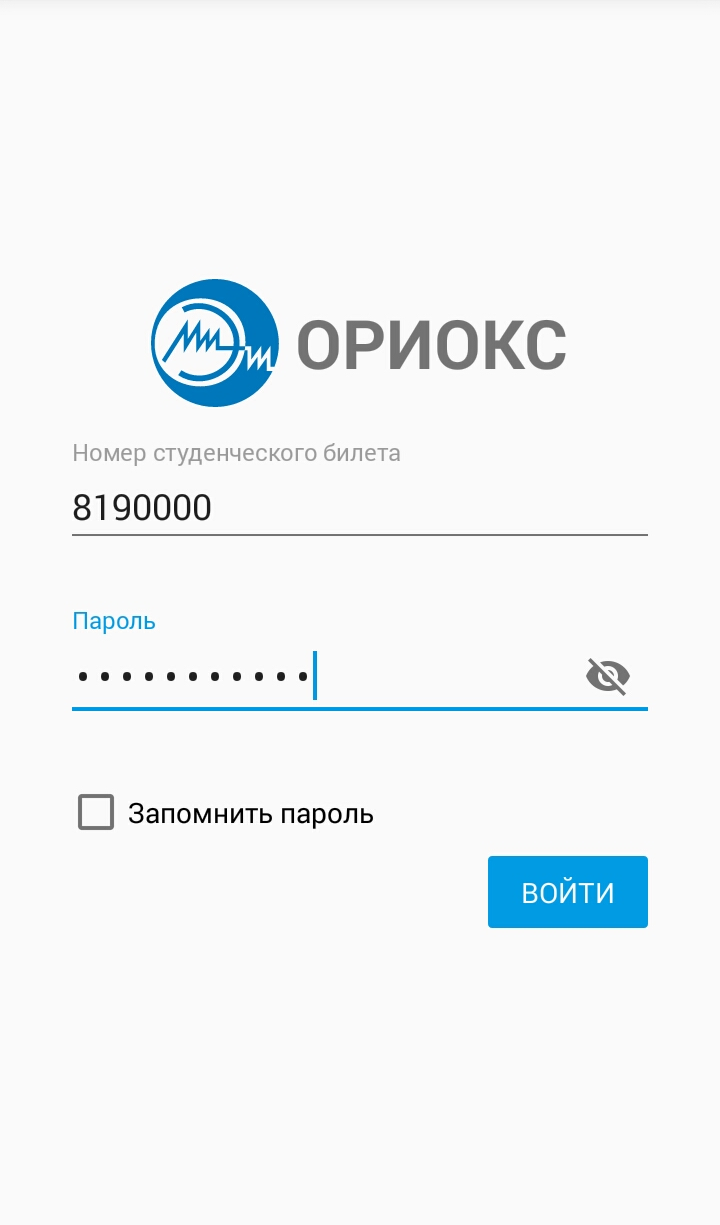
\includegraphics[width=\textwidth]{inc/img/app_auth.png}
    \caption{Экран авторизации}
    \label{fig:auth}
  \endminipage\hfill
  \minipage[t]{0.48\textwidth}
    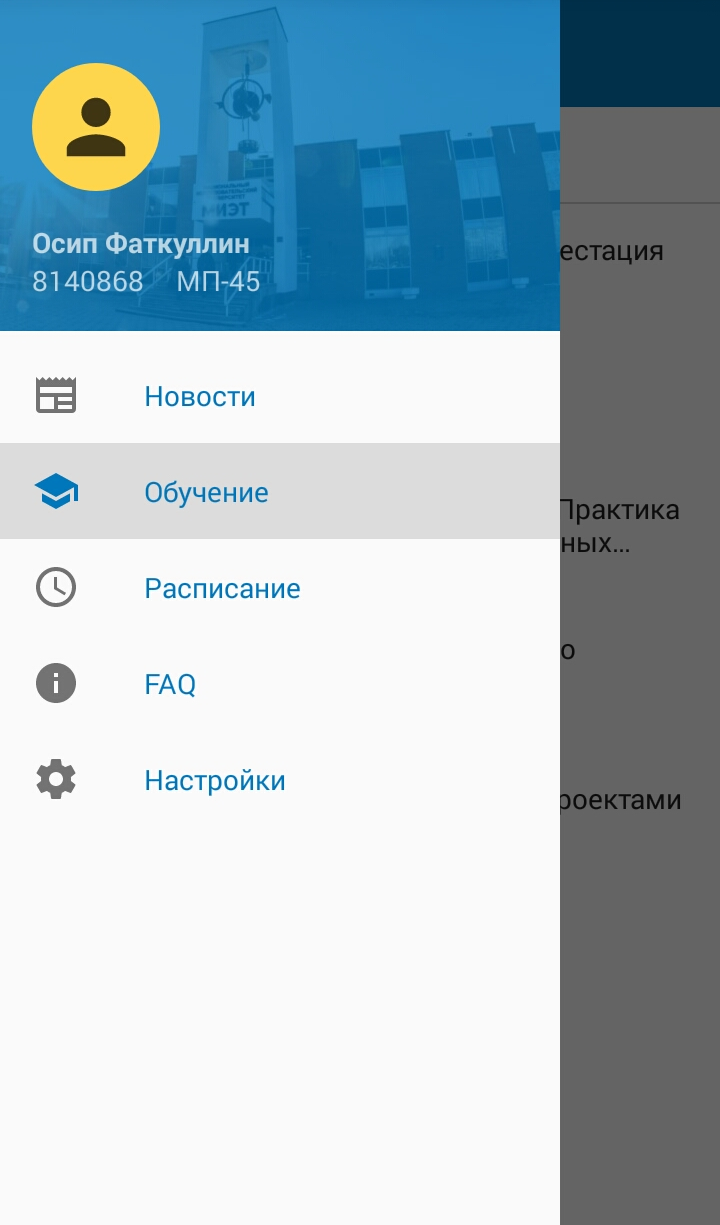
\includegraphics[width=\textwidth]{inc/img/app_menu.png}
    \caption{Экран с открытым главным меню}
    \label{fig:menu}
  \endminipage
\end{figure}

\subsection*{Просмотр данных}
Однотипные данные расположены на разных экранах.
Выбор экрана осуществляется при помощи главного меню приложения (рис.~\ref{fig:menu})
После нажатия на необходимый пункт меню, открывается экран с соответствующими данными.
Данные можно принудительно обновить, при помощи жеста ``свайп вниз''.

При отсутствии соединения и данных в кэше отображается пустое состояние "--- картинка, символизирующая выбранный пункт меню и надпись ``Пусто''.
